%Skrevet Af David
\section{Receiver} \label{Rx}
Receiveren modtager et signal fra ZeroCross detectoren, når der er et 120khz signal på nettet, og derefter læser den fra bitstreamen som indeholder dataene fra *Ref Treansmitteren?*

Klassen har en indbygget debugging-funktion, som udnytter \texttt{RxUART} klassen til at "sladre" om hvad der foregår. Debugging kan aktiveres ved at sætte konstanten \texttt{debugging} til \texttt{true}. Dette hjælper os rigtig meget under implementering da vi kan se helt precise, hvor langt den er nået i modtagelsen af data.

\subsection{Rx10 klassen (David)}

\subsubsection{waitMs()}

Denne hjælpemetode er til for at være sikker på at ramme midt i dataen for en given nulgennemgang.
Da disse er 1 ms lange, vil vi læse 0.5 ms efter nulgennemgangen.
På denne måde er vi mest muligt sikre på at ramme dataen, hvis nu timingen skulle skride en smule.

Metoden fungerer ved at starte timer2 på 0.5 ms, dette er regnet ud ud fra følgende udregninger:

\begin{align*}
t &= \frac{1}{f_{osc}} N (C - 1)\\
 &= \frac{1}{3.6864 \text{MHz}} 64 (29 - 1) \\
 &= 0.5 ms
\end{align*}

Metoden er testet ved at sætte et ben lavt før og højt igen efter metoden og dette er målt med Analog Discovery i Figur \ref{fig:RxwaitMStest}. 
Det ses at timingen passer meget godt med 0.5 ms.

\begin{figure}[h]
\centering
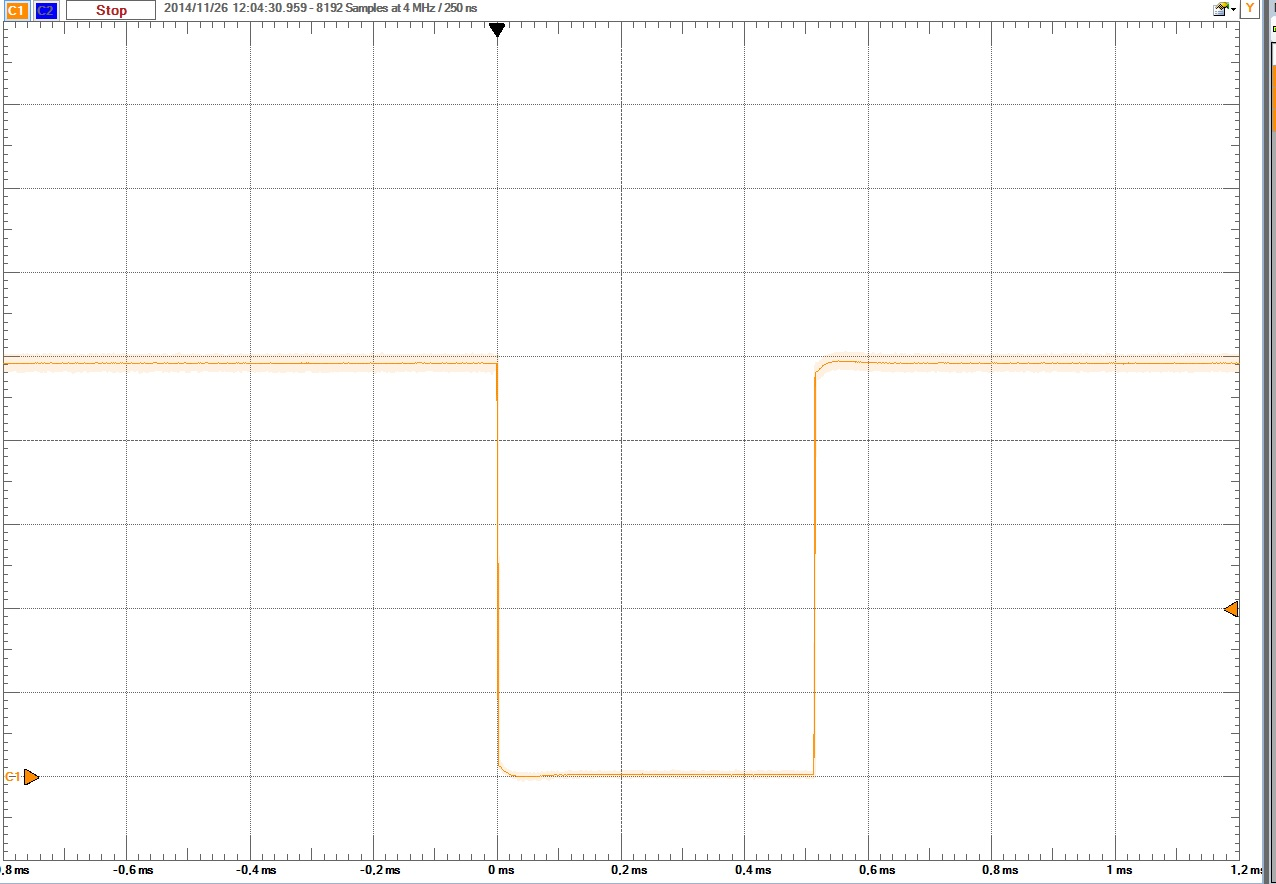
\includegraphics[width=\textwidth]{../Implementering/SW_implementering/Receiver/Rx10}
\caption{Måling af waitMs() metoden.}
\label{fig:RxwaitMStest}
\end{figure}

\subsubsection{interruptHandler()}

Hjælpemetode til at håndtere interrupts fra \texttt{zeroCrossDetected}.

Metoden tjekker i første omgang på hvert interrupt om den har modtaget start-koden fra X10 protokollen (se side X). %TODO indsæt reference til protokollen)

\begin{lstlisting}[caption=Der ventes 0.5 ms og der tjekkes efter startbit.]
	waitMs(); // wait 0.5 ms
	buffer = buffer << 1; // Make rooms the next bit
	buffer |= ( PINA & 0b00000001 ); //Adds the bit in the buffer
	PORTC = ~buffer;

	if (!start){
		if ( ( buffer & 0b00011111) == 0b00001110 ){
			start = true;
			pattCount = 2;
			buffCount = 7;
			if (debugging){
				myRxUART->sendString("New command!\n\r");
			}
		}
	}
\end{lstlisting}

Når start-koden er fundet, sættes \texttt{start} til \texttt{TRUE} og \texttt{pattCount} samt \texttt{buffCount} initieres. 
De efterfølgende otte nulgennemgange fyldes bufferen med data fra \texttt{bitstream}.
Herefter tjekkes det om dataen er valid i forhold til protokollen (så at en høj nulgennemgang efterfølges af en lav og vice versa).
Er protokollen overholdt oversættes dataen og gemmes i en variabel.

\begin{lstlisting}
if (checkData(buffer)){
	if ( pattCount == 2){ // checks if it is in pattern house
		house = translate(buffer);
		buffCount = 7;
			
		if (debugging){
			myRxUART->sendString("HouseCode: ");
			myRxUART->sendNumber(translate(buffer));
			myRxUART->sendString("\n\r");
		}
	...		
	}
	...
else{
	start = false;
	if (debugging){
		myRxUART->sendString("Invalid data!\n\r");	
	}	
}				
\end{lstlisting}

Dette gentages for tre fyldte buffere (24 interrupts/nulgennemgange), hvorefter der forventes 6 tomme nulgennemgange.
Er dette også iorden kontrolleres de næste 24 nulgennemgange om de matcher de foregående, som indeholdte data omkring Actionen.
Hvis disse også er okay, ventes der på en slutkode, som beskrevet i protokollen.
Er der fejl i blot én af ovenstående check kasseres alt og der ventes igen på start-koden.

Under processen overvejede vi også at lave en form for fejlhåndtering, da dette ikke giver mening i forhold til at vi kun har énvejskommunikation og kun dobbelttjekker data. Vi ville ikke risikere at kommandoer gik igennem og blev fortolket forkert.

\subsubsection{translate(unsigned char zeroCrossingCode)}

Er implementeret ved at tage de bits vi er interesserede i og gemme dem over i en lokal variabel, som herefter returneres.

\begin{lstlisting}
unsigned char Rx10::translate( unsigned char zeroCrossingCode ){
	char temp = 0;
	temp = temp | (0b00000001 & (zeroCrossingCode >> 1) ); // Shifts bit 1 into to temp
	temp = temp | (0b00000010 & (zeroCrossingCode >> 2) ); // Shifts bit 2 into to temp and so on.
	temp = temp | (0b00000100 & (zeroCrossingCode >> 3) );
	temp = temp | (0b00001000 & (zeroCrossingCode >> 4) );
	return temp;
}
\end{lstlisting}

\subsection{Receiver control klassen (David og Lasse)}

Receiver klassen fungerer ved, at Rx10 klassen kalder en funktionen \textit{Input()}, med 3 chars, (\textit{houseCode}, \textit{unitCode} og \textit{command}) som parametre. 
Først tjekker funktionen om \textit{houseCode} er lig nul, da dette er en global commando som betyder sluk alt. Dernæst tjekker den om \textit{houseCode} og \textit{unitcode} passer til den respektive receiver. Hvis disse passer til receiveren, vil funktionen, afhængig af kommandoen kalde en funktion i lampe klassen via en pointer til denne.